\documentclass[output=paper, 
colorlinks,
citecolor=brown,
newtxmath
]{langscibook} 
\bibliography{localbibliography}



\author{Rafael Ignacio Zurita\affiliation{Universidad Nacional del Comahue}}
\title{Introducción a PSE2020}  
\abstract{Uno de los avances más sorprendentes de las últimas décadas ha sido el ascenso de las computadoras a una posición en donde nuestras vidas dependan en gran medida de ellas. Existen en un hogar diez o cien veces más computadoras que personas, las cuales trabajan silenciosamente sin que sus habitantes noten su existencia. En este capítulo introducimos el concepto de sistema embebido y dónde se los puede encontrar. También se explica que es la programación embebida y presentaremos las diferencias con respecto a la programación de software general. Por último, indicaremos los detalles por los cuales el lenguaje de programación C es el más ampliamente utilizado en el desarrollo de estos sistemas.

\keywords{sistema embebido, sistema de tiempo real, lenguaje de programación C}
}

% add all extra packages you need to load to this file  
\usepackage{tabularx} 

%%%%%%%%%%%%%%%%%%%%%%%%%%%%%%%%%%%%%%%%%%%%%%%%%%%%
%%%                                              %%%
%%%           Examples                           %%%
%%%                                              %%%
%%%%%%%%%%%%%%%%%%%%%%%%%%%%%%%%%%%%%%%%%%%%%%%%%%%% 
%% to add additional information to the right of examples, uncomment the following line
% \usepackage{jambox}
%% if you want the source line of examples to be in italics, uncomment the following line
% \renewcommand{\exfont}{\itshape}
% \usepackage{./langsci/styles/jambox}
\usepackage{./langsci/styles/langsci-lgr}
\usepackage{./langsci/styles/langsci-osl}
\usepackage{langsci-optional}
% \usepackage{langsci-gb4e}
\usepackage{langsci-cgloss}

\usepackage[linguistics]{forest}

\makeatletter
\let\thetitle\@title
\let\theauthor\@author 
\makeatother

\newcommand{\togglepaper}[1][0]{ 
%   \bibliography{../localbibliography}
  \papernote{\scriptsize\normalfont
Esta es una obra derivada oficialmente autorizada por O'Reilly(*) para la materia "Programación de Sistemas Embebidos" de la Facultad de Informática, Universidad Nacional del Comahue. \\ Detalles de la autorización oficial y sus modificaciones al final del capítulo. \\ Libro original: Programming Embedded Systems with C and GNU Development Tools,
Second Edition, by Michael Barr and Anthony Massa. Copyright 2007 O'Reilly Media, Inc., 978-0-596-00983-0
%    \theauthor.
%    \thetitle. 
%    To appear in: 
%    Change Volume Editor \& in localcommands.tex 
%    Change volume title in localcommands.tex
 %   Berlin: Language Science Press. [preliminary page numbering]
  }
 % \pagenumbering{roman}
  \setcounter{chapter}{#1}
  \addtocounter{chapter}{-1}
}


\usepackage[spanish]{babel}
\usepackage[bottom]{footmisc}

% \IfFileExists{../localcommands.tex}{%hack to check whether this is being compiled as part of a collection or standalone
%   % add all extra packages you need to load to this file  
\usepackage{tabularx} 

%%%%%%%%%%%%%%%%%%%%%%%%%%%%%%%%%%%%%%%%%%%%%%%%%%%%
%%%                                              %%%
%%%           Examples                           %%%
%%%                                              %%%
%%%%%%%%%%%%%%%%%%%%%%%%%%%%%%%%%%%%%%%%%%%%%%%%%%%% 
%% to add additional information to the right of examples, uncomment the following line
% \usepackage{jambox}
%% if you want the source line of examples to be in italics, uncomment the following line
% \renewcommand{\exfont}{\itshape}
% \usepackage{./langsci/styles/jambox}
\usepackage{./langsci/styles/langsci-lgr}
\usepackage{./langsci/styles/langsci-osl}
\usepackage{langsci-optional}
% \usepackage{langsci-gb4e}
\usepackage{langsci-cgloss}

\usepackage[linguistics]{forest}

%   \makeatletter
\let\thetitle\@title
\let\theauthor\@author 
\makeatother

\newcommand{\togglepaper}[1][0]{ 
%   \bibliography{../localbibliography}
  \papernote{\scriptsize\normalfont
Esta es una obra derivada oficialmente autorizada por O'Reilly(*) para la materia "Programación de Sistemas Embebidos" de la Facultad de Informática, Universidad Nacional del Comahue. \\ Detalles de la autorización oficial y sus modificaciones al final del capítulo. \\ Libro original: Programming Embedded Systems with C and GNU Development Tools,
Second Edition, by Michael Barr and Anthony Massa. Copyright 2007 O'Reilly Media, Inc., 978-0-596-00983-0
%    \theauthor.
%    \thetitle. 
%    To appear in: 
%    Change Volume Editor \& in localcommands.tex 
%    Change volume title in localcommands.tex
 %   Berlin: Language Science Press. [preliminary page numbering]
  }
 % \pagenumbering{roman}
  \setcounter{chapter}{#1}
  \addtocounter{chapter}{-1}
} 
%\togglepaper[1]
% }{}

\begin{document}

\selectlanguage{spanish}

\chapterfont{\Large\color{LightBlue}} 
%\chapternumberfont{\large} 
%\chaptertitlefont{\Large}
\chapter*{ Programación de Sistemas Embebidos 2020: Introducción}

\begingroup
\let\clearpage\relax
\cleardoublepage
\hypersetup{linkcolor=blue}
\tableofcontents*
\endgroup


\footnote{\scriptsize\normalfont Esta es una obra derivada oficialmente autorizada por O'Reilly(*) para la materia "Programación de Sistemas Embebidos" de la Facultad de Informática, Universidad Nacional del Comahue. \\ Detalles de la autorización oficial y sus modificaciones al final del capítulo. \\ Libro original: Michael Barr. Programming Embedded Systems in C and C++. ISBN-13: 978-1565923546
ISBN-10: 1565923545. O'Reilly }

{\def\addcontentsline#1#2#3{}\maketitle}



\hfill\begin{minipage}{0.8\linewidth} \footnotesize
I think there is a world market for maybe five computers.
—Thomas Watson, Chairman of IBM, 1943 \\
\\
There is no reason anyone would want a computer in their home.
—Ken Olson, President of Digital Equipment Corporation, 1977 \\
\end{minipage}




% \togglepaper[0]

\section {¿Qué es un sistema embebido?}

Un sistema embebido es una combinación de hardware y software fabricado para realizar una única función. La mayoría de las veces, además de una o más computadoras, un sistema embebido contiene también partes adicionales electrónicas, mecánicas y/o tal vez químicas. 
Un buen ejemplo es el horno microondas, un smartphone o el sistema de inyección electrónica de un auto.
Casi todo sistema digital de un hogar contiene uno, y billones de estos sistemas en están en uso 
cada día, pero pocas personas se dan cuenta que un procesador de computadora y software están
involucrados en el control del sistema (y son quienes realmente están cocinando).



El diseño de un sistema embebido para realizar una función específica es diferente al de una
computadora personal, aún si el hardware es similar. Una computadora personal no está diseñada
para realizar diferentes tareas, y muchas personas utilizan el nombre de computadora de propósito-general
para que la distinción sea clara. Una vez fabricada, una PC tiene un destino indefinido; 
ya que el fabricante no conoce qué hará el cliente con la máquina. Un consumidor podría utilizar
la PC para instalar un servidor de red, otro podría usarla exclusivamente para jugar videojuegos,
y un tercero podría utilizar su computadora para escribir su próxima gran Novela de ciencia ficción.


Frecuentemente, un sistema embebido es un componente de un sistema mayor. Por ejemplo, 
los autos y camiones modernos contienen decenas de sistemas embebidos. Un sistema controla el sistema de frenos anti-bloquenates, otro monitorea y controla la emisión del vehículo, 
y un tercero muestra en pantalla información general del auto al conductor.  Algunos fabricantes de
autos de lujo incorporan en sus publicidades la cantidad numerosa de procesadores que contiene
el auto. Para este caso particular, la mayoría de los sistemas embebidos en un auto
están interconectados a través de una red de comunicaciones.



Un detalle que vale la pena mencionar es que las PC se comunican (interfacing) con 
muchos sistemas embebidos. Por ejemplo, una computadora personal tiene un teclado y un mouse,
los cuales son sistemas embebidos. Estos periféricos contienen un microcontrolador (el cual
a su vez contiene una CPU) que controlan el periférico y se comunican con la computadora.
Su software (usualmente llamado firmware) fue desarrollado para realizar una función.
Otro ejemplo es un disco pen drive USB (USB disk drive), el cual contiene una memoria NAND flash,
un oscilador, y un microcontrolador que controla la memoria flash y se comunica con la PC
via USB. Los demás periféricos de la PC (impresoras, pantallas, cámaras, etc) también
contienen un sistema embebido, y su función específica puede ser expresada utilizando
una única sentencia.

La existencia de un procesador y de software en un sistema embebido suele estar presente sin
ser notado por el usuario del dispositivo. Tal es el caso de un parlante bluetooth, un horno microondas,
o un receptor de TV satelital, por citar algunos ejemplos. En muchos casos es aún posible construir
un dispositivo con una funcionalidad equivalente, que no contiene un procesador y software. 
Esto podría llegar a ser desarrollado reemplazando el procesador y su software con un circuito integrado
(IC) que realiza la misma funcionalidad en hardware. De cualquier manera, la combinación
procesador-software típicamente ofrece mas flexibilidad que un diseño exclusivo en hardware. 
Utilizar un procesador y software en un sistema embebidos es usualmente mucho mas fácil, mas barato y 
consume menos energía.

\subsection {Historia y Futuro}

El primer sistema embebido no apareció hasta después de 1971, si nos guiamos por la
la definición presentada anteriormente En ese ańo Intel introdujo el primer microprocesador en el mundo
que fue plasmado en un chip individual. Ese chip, el 4004, fue diseñado para ser utilizado 
en una familia de calculadoras diferentes, producidas por una compañía Japonesa llamada Busicom.
En 1969, Busicom le preguntó a Intel si podría diseñar un conjunto de circuitos integrados,
uno para cada una de sus calculadoras. El 4004 fue la respuesta de Intel. En vez de diseñar
hardware específico para cada calculadora, Intel propuso un circuito de propósito-general
que podría ser utilizado a través de toda la línea de calculadoras. Este procesador de propósito-general
fue diseñado para leer y ejecutar un conjunto de instrucciones almacenadas en un chip de memoria
externo al procesador. La idea de Intel fue que el software le daría a cada calculadora
un conjunto único de características, y que el este estilo de diseño ayudaría al corazón de su 
negocio que fueron los chips de memoria.



El microprocesador fue un éxito, y su utilización se incrementó continuamente en la siguiente
década. Las primeras aplicaciones embebidas incluyeron sondas espaciales no tripuladas, 
semáforos computarizados y sistemas de control de vuelo de los aviones.
En las décadas de 1980 y 1990, los sistemas embebidos estuvieron presentes silenciosamente
en la era de las microcomputadoras, y luego hicieron que los microprocesadores
pasaran a ser parte de nuestras vidas personales y profesionales.
La mayoría de los dispositivos electrónicos en nuestras cocinas (las máquinas para fabricar pan, la procesadora,
el hornos de microondas), en el living (televisores, equipos de música, controles remotos) y 
en nuestros trabajos (impresoras láser, tarjetas RFID para ingreso, máquinas expendedoras de café,
cajas registradoras, lectores de tarjetas de crédito) son sistemas embebidos.
En el 2006 se utilizaron más de 6 mil millones de microprocesadores nuevos. 
De ese número, menos del 2 por ciento (o aproximadamente 100 millones) de estos microprocesadores 
se utilizaron en computadoras personales, el resto fue destinado a sistemas embebidos.


Es inevitable que el número de sistemas embebidos continúe aumentando año tras año,
ya que nuevos dispositivos se incorporan día a día a nuestras vidas: interruptores de luz y termostatos 
que están conectados en red y pueden ser controlados de forma inalámbrica por nuestros smartphones,
sistemas inteligentes de airbags que no se activan cuando hay niños o adultos pequeños, 
dispositivos médicos de monitoreo que pueden notificar a un médico si las condiciones 
fisiológicas de un paciente se encuentran en niveles críticos, marcapasos de corazón que deben
activarse con restricciones de tiempo muy rigurosas, y sistemas de navegación 
en el tablero que le informan sobre la mejor ruta hacia su destino en las condiciones de 
tráfico actuales. 
Claramente, la demanda por ingenieros que poseen las habilidades y las ganas de diseñar 
la próxima generación de sistemas embebidos está vigente, y lo estará por mucho tiempo.




\subsection {Sistemas de Tiempo Real} 



Una subclase de sistemas embebidos que merece una introducción son los sistemas de tiempo real,
los cuales son sistemas con restricciones de tiempo de repuesta.
La función de un sistema en tiempo real se define, en parte, por su capacidad para hacer
ciertos cálculos o decisiones de manera oportuna. Estos cálculos o actividades 
tienen plazos de finalización específicos.


\begin{figure}
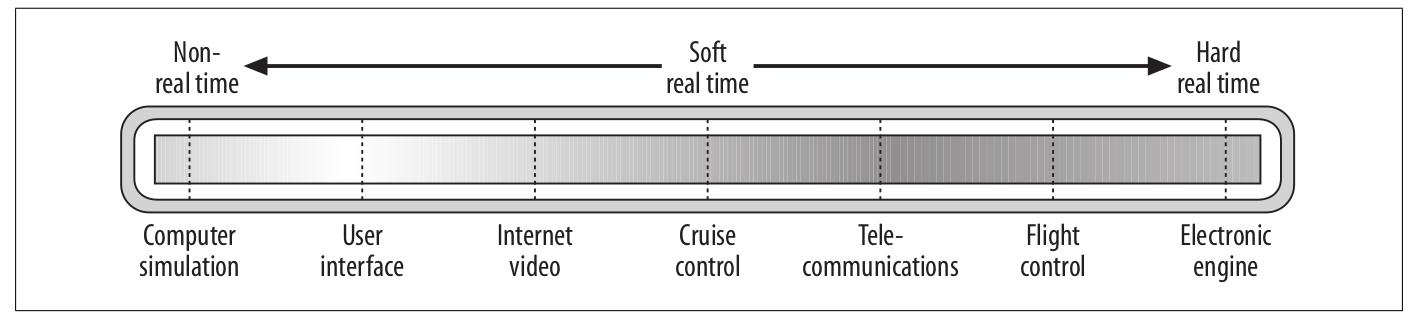
\includegraphics[scale=0.25]{images/real-time-system.jpg}
\caption{Un rango de ejemplos de sistemas de tiempo real}
\label{fig:sist-tiemp-real}
\end{figure}


Existen al menos en la literatura dos categorías de sistemas de tiempo real.
La distinción crucial entre estos radica en lo que sucede si el sistema respondió o no antes
del tiempo definido estricto de respuesta.
Por ejemplo, si el sistema de tiempo real es parte del sistema de control de vuelo de un avión, 
la vida de los pasajeros y la tripulación puede estar en peligro si el sistema no logra
producir la salida antes del tiempo límite (missed deadline).

Si en cambio el sistema está involucrado en la comunicación satelital, el daño podría 
limitarse a la pérdida de un solo paquete de datos (que puede tener o no consecuencias 
catastróficas dependiendo de la aplicación y el esquema de recuperación de errores). 
Si las consecuencias son graves, los sistemas de tiempo real se especifican (y se categorizan)
como sistemas de tiempo real duro (hard real time systems). En esta categoría, si el sistema falla una única vez
en responder antes del tiempo límite (y aún si lo hizo bien por billones de veces) se dice que el 
sistema falló, y no es de tiempo real duro.
En el otro extremo se define la categoría de los sistemas de tiempo real blandos (soft real time systems).
En esta categoría, los tiempos límites de respuesta existen en la especificación, pero para
ciertos eventos está permitido no cumplir el plazo de tiempo para una respuesta, y por lo tanto
el sistema no falló si eso sucede.
La Figura \ref{fig:sist-tiempo-real} muestra algunos ejemplos de sistemas de tiempo real duros y blandos.







En el diseño de un sistema de tiempo real no se trata simplemente de la
velocidad de respuesta. Los plazos para los sistemas en tiempo real varían; 
un tiempo límite puede estar en el orden de los milisegundos, mientras que otro 
a una hora de distancia. El principal objetivo de un sistema en tiempo real es
que garantice que siempre se cumplen los plazos estrictos del sistema. 
Para lograr esto, el sistema debe ser predecible.


La arquitectura del software embebido y su interacción con el hardware juegan 
un papel clave para garantizar que los sistemas de tiempo real cumplan con sus plazos. 
En el diseño del software se debe decidir si el acceso a los dispositivos con E/S programada
(polling) es suficiente, o si se debe utilizar interrupciones, y qué prioridades 
se deben asignar a las diversas tareas y a las rutinas de atención de interrupciones. 
Un análisis adicional debe hacerse: entender los requerimientos de rendimiento del peor caso
(o de varios si los hubiese).


El diseñador de un sistema en tiempo real (o su equipo si el sistema es complejo) debe ser
muy eficas en su labor (debe prestar mayor atención y cuidado al diseño de un sistema
de tiempo real que de uno que no lo es); 
ya que debe 
garantizar el funcionamiento confiable del software y hardware en todas 
las condiciones posibles. Y, en la medida en que las vidas de las personas dependan 
de la ejecución adecuada del sistema, esta garantía debe estar respaldada por 
cálculos de ingeniería y documentación descriptiva completa.




\section {Variaciones sobre el mismo Tema}




A diferencia del software diseñado para PC, el software embebido no puede ser ejecutado
en otros sistemas embebidos sin realizar una modificación considerable. Esto se debe 
principalmente a la increíble variedad de hardware que se utiliza.
El hardware de cada sistema embebido está diseñado específicamente para la aplicación, 
a fin de mantener los costos del sistema lo más bajo posible. Como resultado, 
se elimina toda la circuitería innecesaria, y los recursos de hardware se 
aprovechan al máximo en la medida de lo posible.
En esta sección, se detallan las características de hardware que son comunes 
a todos los sistemas embebidos y por qué hay tanta variedad con respecto a casi 
todo lo demás. Existen técnicas de desarrollo inicial para minimizar el impacto de 
los cambios de software si el hardware llega a cambiar, de modo que no deberían
hacerse modificaciones en todas las capas del software.



\subsection {Componentes del Sistema Comunes}


Por definición, todos los sistemas embebidos contienen un procesador y software, 
pero ¿qué otras características tienen en común?. En realidad, para poder tener software, 
se debe contar con algún lugar donde almacenar el código ejecutable y también
memoria temporal para las variables y el estado del programa en tiempo de ejecución. 
Por lo que casi todos los sistemas embebidos incluyen una memoria de solo lectura (ROM) 
para almacenar el programa, y una memoria de acceso aleatorio (RAM), para la vida
de las variables en tiempo de ejecución. Si solo se requiere una pequeña cantidad 
de memoria entonces usualmente ambas memorias están contenidas dentro del mismo chip junto al
procesador.
De lo contrario, uno o ambos tipos de memoria residen en chips de memoria externos.

Todos los sistemas embebidos también presentan entradas y salidas. Por ejemplo, 
en nuestro ejemplo de horno microondas, las entradas son los botones en el panel 
frontal y una sonda de temperatura, y las salidas son la pantalla (DISPLAY) 
la radiación de microondas, y su control. Las salidas de un sistema embebido es 
casi siempre una función de sus entradas plus otros factores (tiempo transcurrido, 
temperatura actual, etc.). La teoría de control (al menos en su forma
más común utilizada, llamada PID control)
se estudia en varias ramas de ingeniería, y se utiliza en el diseño de las 
funciones de salida de un sistema embebido. Las entradas al sistema generalmente toman 
la forma de sensores y sondas, señales de comunicación o perillas, y botones de control. 
Las salidas son típicamente pantallas, señales de comunicación o cambios en el mundo físico.

En la Figura \ref{fig:hardware-basico} puede observarse el diagrama de bloques
del hardware de una computadora embebida típica.
Toda la columna de la derecha son periféricos que generalmente,
en muchas computadoras embebidas, se encuentran internos en el mismo chip
junto al procesador. Estos periféricos internos se utilizan 
para interconectar el sistema con otros dispositivos externos. En nuestro ejemplo
del microondas, el sensor de temperatura podría conectarse al ADC,
los botones a puertos GPIO, la pantalla LCD al SPI y el 
controlador de radiación externo al PWM.
Todos los periféricos externos mencionados tendrán que tener
esas interfaces de conexiones por hardware (una señal analógica,
switches, LCD con interfaz SPI, controlador de radiación
que admita una señal PWM de control).


\begin{figure}[h]
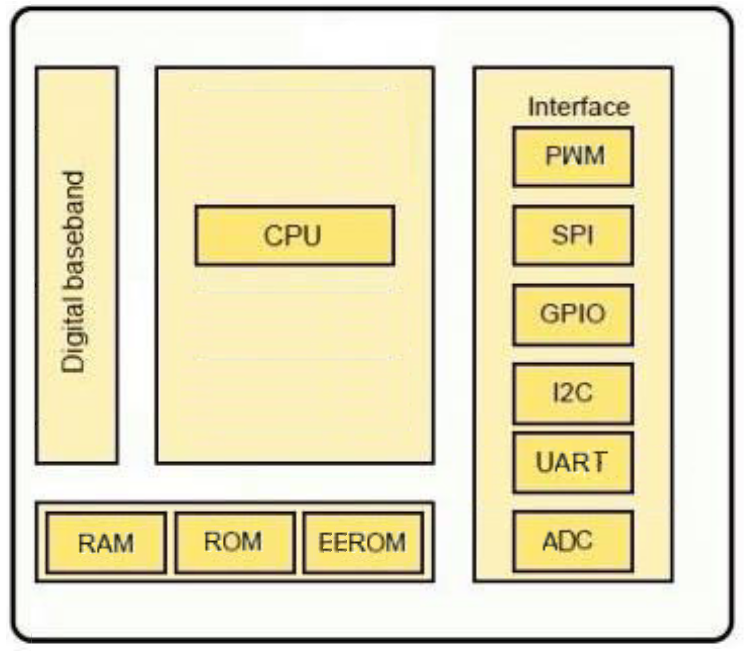
\includegraphics[scale=0.25]{images/hardware-basico2.png}
\caption{Una computadora para sistemas embebidos: CPU, RAM y E/S}
\label{fig:hardware-basico}
\end{figure}




Con la excepción de estas pocas características comunes, el resto del hardware en un sistema
embebido es generalmente único y, por lo tanto, requiere un software único. 
Esta variación es el resultado de muchos criterios de diseño competitivos de los fabricantes.
La Figura \ref{fig:sistema-embebido-basico} proporciona un par de diagramas de alto nivel 
posibles, que podrían implementarse en un sistema embebido genérico.


\begin{figure}[h]
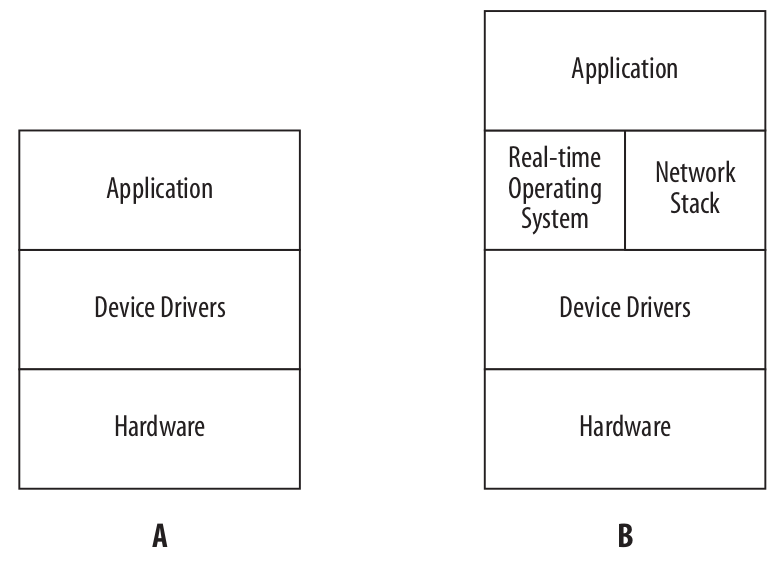
\includegraphics[scale=0.3]{images/sistema-embebido-basico.png}
\caption{(a) y (b) Diagramas de los componentes de dos sistemas embebidos}
\label{fig:sistema-embebido-basico}
\end{figure}


Tanto el diagrama de software embebido básico en la Figura \ref{fig:sistema-embebido-basico} (a) como el diagrama de software más complejo 
en la Figura \ref{fig:sistema-embebido-basico} (b) contienen bloques muy similares. El bloque de hardware es común en ambos diagramas.
Los controladores de dispositivo (drivers) son módulos de software que contienen la funcionalidad 
para operar (controlar) los dispositivos de hardware (periféricos). Estos controladores
eliminan la necesidad de que la aplicación sepa cómo controlar cada pieza de hardware, además permiten su reuso. 
Cada controlador individual de dispositivo normalmente necesitaría saber solo cómo controlar su dispositivo de hardware y no varios. 
Por ejemplo, para un horno microondas, tendríamos que desarrollar o incorporar al menos cuatro drivers distintos: 
los controladores del teclado, la pantalla, la sonda de temperatura y el control de radiación.
Si el sistema requiere de más funcionalidades a veces es necesario incluir capas 
de software adicionales para ayudar con cada funcionalidad adicional. 
En este ejemplo, el diagrama complejo incluye un sistema operativo en tiempo real (RTOS) 
y una pila de red. El RTOS usualmente no es un sistema operativo completo, sino que más
bien son módulos de software que ayudan al programador a separar la funcionalidad 
de la aplicación en tareas diferentes para una mejor organización del software,
y que el sistema sea más receptivo. 
La pila de red también se suma como funcionalidad extra al sistema básico; 
un horno de microondas podría usar la red para que aparezca un mensaje 
en su computadora de escritorio cuando su almuerzo esté listo.





Las responsabilidades de la capa de software de aplicación son las mismas 
en los diagramas de software integrados básicos y complejos. 
En un horno microondas, la aplicación procesa las diferentes entradas 
y controla las salidas en función de lo que el usuario ordenó.
Notará que el software en la Figura \ref{fig:sistema-embebido-basico} está representado por bloques 
discretos apilados uno encima del otro con bordes fijos. Esto se hace deliberadamente, 
para indicar que existe una separación clara de las diferentes capas funcionales 
de software que conforman el firmware completo. 
Mantener estas capas de software en módulos diferentes con interfaces bien definidas para 
que las capas vecinas pueden comunicarse, le ayudará a desarrollar software embebido 
que sea claro, limpio, fácil de leer y portátil.



\subsection {Requerimientos que Afectan a las Decisiones de Diseño}



Cada sistema embebido debe cumplir un conjunto de requisitos completamente 
diferente, cualquiera de los cuales puede afectar a las decisiones realizadas durante el 
desarrollo del producto. Por ejemplo, si el sistema debe tener un costo de producción menor a 
\$ 10, otras caracterísitas usualmente deseables, como el consumo energético o
la confiabilidad del sistema, podrían necesitar ser sacrificadas para alcanzar ese objetivo.
Por supuesto, el costo de producción es solo una de las posibles restricciones 
bajo las cuales trabajan los diseñadores de hardware embebido. Otros requisitos comunes 
de diseño son:



\subsubsection {Rendimiento del procesador}


Es la carga de trabajo que puede computar el chip principal. 
Una forma común de comparar el rendimiento de procesamiento entre dos procesadores 
es la clasificación de millones de instrucciones por segundo (MIPS). En general,
si dos implementaciones de procesadores de la misma arquitectura tienen calificaciones 
de 25 MIPS y 40 MIPS respectivamente, se dice que este último es más potente. 
Sin embargo, deben considerarse otras características importantes del procesador. 
Uno es el ancho del camino de datos en la CPU, que varía de 8 a 64 bits. 
Las PC y laptos de hoy en día son de 64 bits (con algunas aún de 32 bits) 
mientras que en la construcción de sistemas embebidos
se utilizan tambien procesadores menos potentes de 8 y 16 bits.
Procesadores de arquitecturas diferentes son díficiles de comparar. Para
realizar una comparación se pueden realizar benchmarks, y medir el tiempo
de ejecución de varios programas. En estas pruebas los programas
fuentes a utilizar para medir el tiempo de ejecución en cada máquina
tienen que ser los mismos. Tambien el ambiente en donde se ejecutan,
si existe software de soporte a más bajo nivel. Por ejemplo, si existe
Linux en los sistemas a comparar, lo mas indicado es utilizar
exactamente la misma versión de la distribución Linux en cada
sistema (si son de diferentes arquitecturas la distribución Linux
debe proveer los paqutes para las diferentes arquitecturas con la misma versión;
si esto no es posible entonces no se podrá realizar la comparación de rendimiento
adecuadamente).
Además ambos sistemas deben tener exactamente la misma instalación y 
configuración (los mismos paquetes en cada sistema).


\subsubsection {Memoria}

La cantidad de memoria (ROM y RAM) que se necesita para almacenar
y ejecutar el software del sistema embebido. Aquí, el diseñador de 
hardware generalmente debe realizar los cálculos necesarios para
estimar de la mejor manera posible por adelantado, y estar preparado para 
aumentar o disminuir la cantidad real a medida que se desarrolla el software. 
La cantidad de memoria requerida también puede afectar a la selección del 
procesador. En general, el ancho del camino de datos y de los buses de un procesador 
establecen el límite superior de memoria a la que se puede 
acceder (por ejemplo, un registro de dirección de 16 bits puede abordar solo 
64 KB ($2^{\text{16}}$) ubicaciones de memoria). \footnote{Procesadores 
con un ancho de bus estrecho generalmente presentan por hardware 
indirecciones u otros trucos para acceder a 
más memoria. Cuanto más estrecho sea el ancho del bus 
más probable es que suceda lo anterior.}

Algunos sistemas embebidos pueden realizar su trabajo
con unos pocos bytes; sin embargo varios miles de bytes es un requisito de
memoria mínimo más común, incluso en un procesador de 8 bits.


\subsubsection {Cantidad de unidades}

Es la cantidad esperada de unidades a fabricar. 
La inversión destinada al desarrollo y producción se verá afectada 
por la cantidad de unidades que se espera fabricar y vender.
Por ejemplo, rara vez tiene sentido desarrollar componentes de 
hardware especializados para un sistema que tendrá un bajo volumen de producción.


\subsubsection {Consumo de energía}

La cantidad de energía utilizada durante la operación. 
Este requerimiento de diseño suele ser extremadamente importante, 
especialmente en dispositivos portátiles alimentados por un batería. 
Una métrica comúnmente utilizada es mW / MIPS (milivatios por MIPS); 
cuanto mayor es este valor se necesitará más potencia para realizar el trabajo. 
Un menor consumo de energía también favorece, usualmente,
al sistema en general (tanto en su diseño como fabricación posterior). Esto
se debe a que el dispositivo generará menos calor, sus
baterías serán más pequeñas, tendrá un peso final menor, 
será mas compacto, y el diseño mecánico será más sencillo.


\subsubsection {Costo de desarrollo}

El costo del proceso de diseño del software y del hardware, conocido como nonrecurring engineering
(NRE). Es una inversión de única vez, y generalmente fija. El presupuesto para
esta inversión tiene directa relación con la producción final. Si el volumen de productos
será muy grande, el NRE puede tener un presupuesto alto. En cambio, para una producción
de bajo volumen puede haber un presupuesto acotado.


\subsubsection {Tiempo de vida}

El tiempo esperado de uso del producto. El tiempo de vida requerido o esperado
afecta a todas las decisiones de diseño, desde la selección de los componentes
de hardware a cuánto es posible invertir en el desarrollo del sistema y su 
producción. La pregunta a responder es : Cuánto tiempo (en promedio) el sistema
debe funcionar? ¿Un mes? ¿Un año? ¿Una década?.



\subsubsection {Confiabilidad}

Este requerimiento indica usualmente la calidad del producto final. 
Si es un juguete para chicos es posible que no tenga que funcionar correctamente el 100 por 
ciento del tiempo, pero tal vez debe ser seguro (partes pequeñas sueltas podrían ser ingeridas por 
un niño menor a 3 años). En cambio, si se trata de un sistema antibloqueo 
de frenos para un automóvil, es necesario que funcione todas las veces
que se necesite, y que lo haga como se requiere.

Además de estos requisitos generales, cada sistema tiene requisitos funcionales 
detallados específicos; que le dan al sistema embebido su identidad única (horno de microondas, marcapasos o consola de juegos).

La Figura \ref{fig:tabla-rango} presenta una tabla con el rango de valores típicos para cada uno de los requisitos de diseño anteriores. 

Las etiquetas bajo, medio y alto tienen fines ilustrativos y no deben tomarse como límites estrictos. 
Un producto real tiene una selección de cada fila. En algunos casos, dos o más de los criterios 
podrían estar vinculados. Por ejemplo, un aumento en la potencia de procesamiento 
requerida podrían generar mayores costos de producción. 
Por el contrario, podríamos pensar que el mismo aumento en la potencia de 
procesamiento tendrá el efecto de disminuir los costos de desarrollo, 
al reducir la complejidad del diseño de hardware y software. 
Por lo tanto, los valores en una columna en particular no necesariamente van juntos.


\begin{figure}
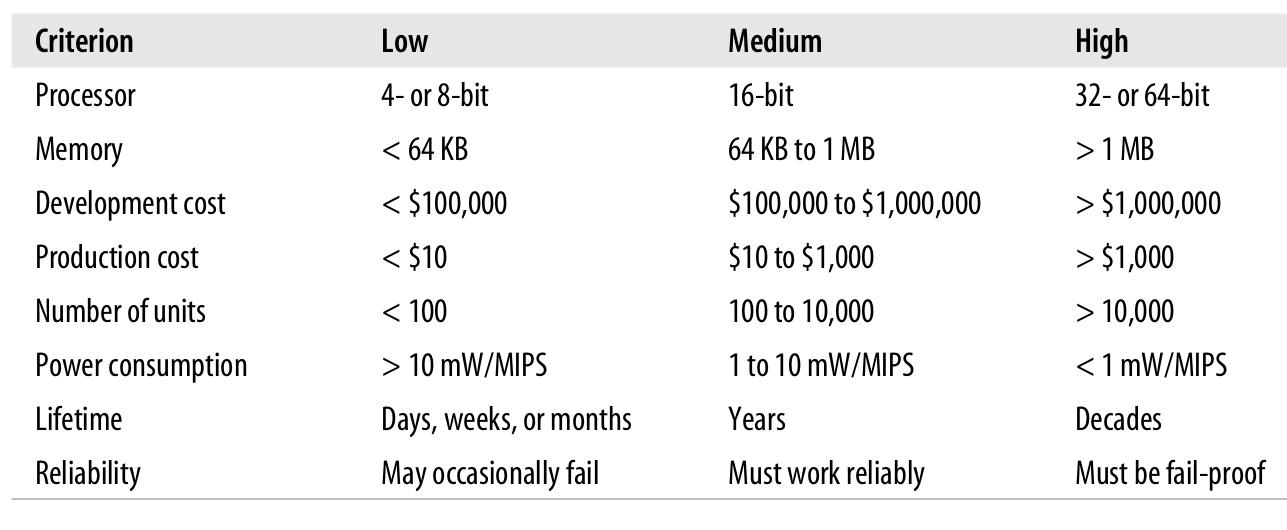
\includegraphics[scale=0.25]{images/requerimientos-comunes.jpg}
\caption{Requerimientos comunes para diferentes sistemas embebidos}
\label{fig:tabla-rango}
\end{figure}



\section {Tres Ejemplos de Sistemas Embebidos}

En esta sección se presentan tres ejemplos de sistemas
embebidos reales, los cuales tienen marcadas
diferencias en sus objetivos y 
requerimientos. Se notará que las diferencias
en sus requerimientos afectan a las decisiones realizadas
en hardware. 

\subsection {Reloj digital}

En la cima actual del camino evolutivo que comenzó con relojes de sol, relojes de agua y relojes de arena está el reloj digital.
Entre sus muchas características están la presentación de la fecha y la hora 
(generalmente al segundo más cercano), la medición de la duración de un evento a la centésima de 
segundo más cercana y la generación de un pequeño sonido molesto al comienzo de cada hora. 
Como resultado, estas son tareas muy simples que no requieren mucha potencia de procesamiento o memoria. 
De hecho, la única razón para emplear un procesador es admitir una gama de modelos y 
características desde un solo diseño de hardware.
El reloj digital típico contiene un procesador de 8 bits simple y económico. Debido a que estos procesadores 
no pueden direccionar mucha memoria, contiene su propia pequeña ROM en el chip. 
Y, si hay suficientes registros disponibles, es posible que esta aplicación 
no requiera RAM en absoluto. De hecho, es probable que todos los componentes 
electrónicos (procesador, memoria, contadores y relojes en tiempo real) sea el único hardware
disponible en el chip.
Los otros elementos de hardware del reloj son las entradas (botones) y las salidas (pantalla y altavoz).

El objetivo de un diseñador de relojes digitales es crear un producto razonablemente 
confiable, y que tenga un costo de producción extraordinariamente bajo. 
Si, después de la producción, se descubre que algunos relojes mantienen un 
tiempo más confiable que los demás, se pueden vender bajo una marca mas cara.
Por lo demás, aún se pueden obtener ganancias vendiendo el reloj a través 
de un canal de venta con descuento. Para las versiones de menor costo, 
los botones del cronómetro o el altavoz podrían eliminarse. 
Esto limitaría la funcionalidad del reloj, pero podría requerir pocos o incluso 
ningún cambio de software. Y, por supuesto, el costo de todo este esfuerzo de 
desarrollo puede ser bastante alto, ya que se amortizará en cientos de miles o 
incluso millones de ventas de relojes.
En el caso del reloj digital, vemos que el software, especialmente cuando está 
cuidadosamente diseñado, permite una enorme flexibilidad en respuesta a un mercado 
rápidamente cambiante y altamente competitivo.

Un tipo de reloj mas actual es el reloj digital inteligente. Este reloj es totalmente
diferente al anterior y puede costar mil veces más. 
Los relojes inteligentes tienen usualmente un microprocesador de 32 bits (arquitectura ARM),
mucha cantidad de RAM para estos dispositivos (por ej. 512MB) y varios
GB de disco. Cuentan con conexión wireless y su software se comunica
con un teléfono inteligente, del cual obtiene mensajes y avisos para comunicar
al usuario a través de una pantalla LCD en el reloj.
En este tipo de relojes el presupuesto de desarrollo es mucho mayor,
porque ya la categoría del hardware a controlar y del software 
a desarrollar es extremadamente compleja.



\subsection {Consola de Vídeo Juegos}

Cuando conectes tu Sony PlayStation 4 a tu smart TV te estás preparando para utilizar decenas de sistemas embebidos.
Las consolas de vídeo juegos pueden llegar a ser más potentes que las PC
de su misma generación; aún si las consolas son relativamente mas baratas que las PC.
Esto se debe a que existe un requisito competitivo de alto poder de cómputo
a un costo bajo de producción. Tales requisitos obligan a los 
diseñadores de las consolas de videojuegos a estar despiertos por las noches.

A las compañías que producen consolas de videojuegos generalmente no les importa 
cuánto cuesta desarrollar el sistema, siempre que los costos de producción del 
producto resultante sean bajos.
Incluso podrían ofrecer la posibilidad, a sus ingenieros, de diseñar un procesador personalizado 
a un costo de desarrollo de millones de dólares cada uno. 
Entonces, aunque puede haber un procesador de 64 bits dentro de la consola 
probablemente no sea el mismo procesador que se encontraría en una 
computadora personal. Con toda probabilidad, el procesador está altamente especializado 
para las demandas de los videojuegos que está destinado a ejecutar.

Debido a que el costo de producción es tan crucial en el mercado de videojuegos 
se deben también realizar ciertos tricks para modificar esos costos. Por ejemplo, los
diseñadores han utilizado la táctica de mover la mayor cantidad de memoria 
y otros dispositivos electrónicos fuera de la 
placa de circuito impreso principal, y han colocado este hardware en los cartuchos de juego. \footnote{Por ejemplo, hace muchos años, Atari y Nintendo 
han diseñado algunos de sus sistemas de esta manera.}
Esto ayuda a reducir el costo de la consola pero aumenta el precio de cada juego. 
Entonces, si bien el sistema podría tener un procesador potente de 64 bits, 
podría tener solo unos pocos megabytes de memoria en la placa de circuito principal. 
La memoria debe ser suficiente para iniciar 
la máquina a un estado desde el cual se puede acceder a la memoria adicional 
contenida en el cartucho del juego. Ni mas memoria ni menos.


Podemos ver, en este ejemplo, que en productos de gran masividad se puede dedicar 
mucho esfuerzo de desarrollo a ajustar cada aspecto del sistema.





\subsection {Mars Rover}

En 1976, dos naves espaciales no tripuladas llegaron al planeta Marte. 
Como parte de su misión, debían recolectar muestras de la superficie marciana, 
analizar la composición química de cada una y transmitir los resultados a los 
científicos en la Tierra. Esas misiones Vikingas fueron impresionantes. 
Siendo que uno está rodeado de computadoras personales que deben reiniciarse 
ocasionalmente, podríamos encontrar casi increíble que hace más de 30 años, 
un equipo de científicos e ingenieros construyeron con éxito dos computadoras 
que sobrevivieron a un viaje de 34 millones de millas y funcionaron 
correctamente durante media década. 
Claramente, la confiabilidad era uno de los requisitos más importantes para estos sistemas.

¿Qué pasa si un chip de memoria falla? ¿O si el software contenía errores y se bloqueaba? 
¿O si se hubiese roto una conexión eléctrica durante el impacto? 
No hay forma de evitar que ocurran tales problemas, y en otras misiones espaciales, 
estos problemas han resultado ser desastrosos. 
Entonces, todos estos puntos potenciales de falla y muchos otros 
tuvieron que ser eliminados agregando circuitos redundantes o 
funcionalidades adicionales:
un procesador adicional aquí, diagnósticos especiales de memoria por allá, 
un temporizador de hardware para reiniciar el sistema si el software se 
bloquea, y así sucesivamente.

Más recientemente, la NASA lanzó la misión Pathfinder. Su objetivo principal era 
demostrar la viabilidad de llegar a Marte con un cierto presupuesto. 
Por supuesto, dados los avances tecnológicos realizados desde mediados de 
los años 70, los diseñadores no tuvieron que quitar muchas características del sistema (como uno esperaría)
para lograr esto. Es posible que hayan reducido un poco la cantidad de 
redundancia, pero aún así le dieron a Pathfinder más poder de procesamiento y memoria
que al anciano Vikingo. El Mars Pathfinder estaba compuesto en realidad 
por dos sistemas embebidos: una nave de aterrizaje y un rover. 
La nave de aterrizaje tenía un procesador de 32 bits y 128 MB de RAM; 
el rover, por otro lado, solo tenía un procesador de 8 bits y 512 KB de RAM. 
Estas elecciones reflejan los diferentes requisitos funcionales de los dos 
sistemas. El costo de producción probablemente no fue un gran problema en 
ninguno de los casos.



\section {La vida como desarrollador de sistemas embebidos}

Veamos ahora brevemente algunas de las cualidades del software embebido, 
que diferencian a los desarrolladores embebidos de otros tipos de desarrolladores de software. 
Un desarrollador de software embebido es aquél que se ensucia las manos acercándose al hardware.

El desarrollo de software embebidos, en la mayoría de los casos, requiere una estrecha interacción 
con el mundo físico: la plataforma de hardware. Decimos \textit{en la mayoría de los casos}
porque hay sistemas embebidos muy grandes que requieren que las personas trabajen 
únicamente en la capa de aplicación del sistema. 
Estos desarrolladores generalmente no necesitan tener ninguna 
interacción directa con el hardware. Cuando se diseñan correctamente, los controladores 
de hardware (software drivers) se abstraen del hardware real de tal modo
que un desarrollador que escribe el software a nivel de aplicación 
no necesita conocer cómo es que aparece un texto en la pantalla, 
sólo que sucede cuando se llama a una rutina particular con los parámetros adecuados.


\subsubsection {Conocimiento del hardware}

El desarrollador de software embebido debe familiarizarse íntimamente con los 
circuitos integrados, las placas de circuito impreso, los buses, y los dispositivos 
que se utilizan para transferir y testear el software embebido sólido (también denominado firmware). 
No se debe sentir temor por los esquemáticos, o tomar una sonda del osciloscopio y 
comenzar a hurgar en el circuito para descubrir qué está sucediendo.



\subsubsection {Código eficiente}

Los desarrolladores de software embebido deben tener en cuenta
cada línea de código fuente, ya que los sistemas embebidos 
están diseñados, generalmente, con el procesador menos potente posible
(pero que cumple con los requisitos de rendimiento del sistema). 
La capacidad de escribir código eficiente es una gran cualidad
que deben poseer los desarrolladores de firmware.



\subsubsection {Interfaces a los dispositivos}

A bajo nivel el firmware es muy especializado, porque cada componente o circuito 
tiene su propia actividad que realizar y, además, su propia forma de realizar esa actividad. 
Los desarrolladores embebidos necesitan saber cómo comunicarse con 
los diferentes dispositivos o periféricos, para tener un control total de los mismos dentro
del sistema. Saber como atender eventos provenientes de periféricos externos es una gran 
parte del desarrollo de software embebido.

Por ejemplo, en un horno microondas, el firmware puede obtener los datos 
del sensor de temperatura leyendo un registro de 8 bits de un 
conversor externo analógico a digital. En otro sistema, los datos 
podrían provenir controlando un bus serie que se conecta al 
circuito del sensor externo a través de un único cable.
Dos maneras distintas en hardware y software en dos sistemas distintos
para una misma funcionalidad de entrada.


\subsubsection {Código robusto}

Un sistema que puede manejar entradas que están fuera del rango
específico de sus requerimientos, y continúe funcionando 
sin problemas, es robuto.
También, en muchos casos, se espera que el sistema embebido funcione durante años.
Este no es un requisito típico para las aplicaciones desarrolladas para PC, Mac o el smartphone (aunque hay excepciones),
pero es importante por el siguiente ejemplo: si luego de un tiempo la única manera de finalizar la
coción en su horno microondas es abriendo la puerta (porque el sistema de reloj o stop automático ya no funciona,
o lo que fuese la causa) entonces es muy probable
que ya no vuelva a comprar un producto de esa marca.





\subsubsection {Recursos mínimos}

En la misma línea de crear un sistema más robusto, el desarrollador
de software embebido se diferencia de otros tipos de desarrolladores
por tener que trabajar con recursos limitados.
Las reglas para desarrollar un firmware son diferentes de las reglas para 
escribir software para una PC. Piense en la gestión de la memoria por ejemplo.
Una aplicación para una PC moderna puede dar por sentado que tendrá acceso a recursos prácticamente ilimitados. Pero en un sistema embebido, se quedará sin memoria si no planifica con anticipación y diseña el software correctamente.
Un desarrollador de software embebido debe calcular cuidadosamente cuantos
recursos consumirá el sistema cuando esté en ejecución, para todos sus estados
(cuanta memoria y cuanto CPU).
Por supuesto, también para que el sistema funcione según 
las especificaciones y sin fallas. Por ejemplo, 
si se utilizan las funciones de asignación de memoria dinámica 
estándar puede que para algún caso particular de entradas
y estado el sistema de memoria esté fragmentado, y deje de funcionar.
Esto requiere un reinicio ya que no tiene lugar para almacenar datos entrantes.

Muy a menudo, se diseña el software de tal manera que al iniciarse
su ejecución se asigna e inicialize toda la memoria que necesita la aplicación
para su funcionamiento. Esta es una asignación estática (se define
en tiempo de compilación).
Esto es más seguro que usar asignación dinámica de memoria, 
aunque no siempre será posible utilizar este método.




\subsubsection {Software reutilizable}

Como mencionamos anteriormente, la portabilidad del código o la 
reutilización del código —desarrollar software para que se pueda compilar
y ejecutar en otra plataforma y arquitectura de hardware— es muy 
útil en la transición a nuevos proyectos. Esto no siempre se puede hacer.
Hemos visto cuán individual es cada sistema embebido. 
De todas maneras, muchos de los módulos de un software embebido
puede diseñarse con interfaces que oculten los detalles del hardware
subyacente. Si esto se logra, gran parte del código podría ser portable.
Por ejemplo, si en su próximo proyecto se utiliza una pantalla LCD 
para la cual se ha desarrollado previamente un controlador, 
puede colocar el código anterior y ahorrar un tiempo importante en el cronograma.



\subsubsection {Herramientas de desarrollo}

Las herramientas que se utilizan a lo largo de una carrera 
como desarrollador embebido serán diferentes de una compañía a otra y, 
a menudo, de un proyecto a otro. Esto significa que necesita
aprender nuevas herramientas a medida que pasen los años.
Por lo general, estas herramientas no son tan potentes 
o fáciles de usar como las que se usan en los entornos
de desarrollo para PC.

Las herramientas de depuración, por ejemplo, pueden variar de plataforma
en plataforma. Tal vez en una tenga simplemente un LED conectado a la placa,
y en otra puede que tenga algo mucho mas completo como un emulador de 
circuito completo (ICE). Esto requiere que, como desarrollador de 
firmware y responsable de depurar 
su código, sea muy ingenioso y tenga un conjunto de técnicas a las que 
pueda recurrir cuando falte el entorno de depuración. 

Estas son solo algunas cualidades que diferencian a los desarrolladores 
de software embebido del resto.



\section {El lenguaje C: un denominador común}

Una de las pocas cosas regulares en la mayoría de los sistemas embebidos es el uso del 
lenguaje de programación C.
Más que ningún otro, C se ha convertido en el lenguaje de los programadores de estos sistemas. 
Este no siempre ha sido el caso, y tal vez no seguirá siéndolo para siempre. 
Sin embargo, en este momento, C es lo más parecido a un estándar en el mundo embebido (en el mundo hobbysta Arduino, sin embargo, el lenguaje utilizado en el ambiente de desarrollo Arduino es C++). Pero en todos los demás casos el denominador común es C. 

Debido a que el éxito del desarrollo de software depende entre otras cosas de seleccionar 
el lenguaje de programación mas indicado, es sorprendente observar que 
un mismo lenguaje ha demostrado ser apropiado para procesadores de 8 y 64 bits; 
en sistemas con muy poca memoria o ninguna (unos pocos bytes) a sistemas
con GBs de RAM; y para equipos de desarrollo compuestos por un sólo desarrollador 
a equipos con una docena de personas o más. 
Sin embargo, esta es precisamente la gama de proyectos en los que C ha prosperado.

El lenguaje de programación C tiene muchas ventajas. 
Es reducido y bastante simple de aprender, los compiladores están disponibles 
para casi todos los procesadores que se usan en la actualidad, y hay un 
gran grupo de programadores de C con experiencia. 
Además, C tiene la ventaja de la independencia del procesador, 
que permite a los programadores concentrarse en algoritmos y aplicaciones 
en lugar de en los detalles de una arquitectura en particular. 
Sin embargo, muchas de estas ventajas también existen 
en otros lenguajes de alto nivel. Entonces, ¿por qué C ha tenido 
tanto éxito aquí y otros no?

Quizás la mayor fortaleza de C, y lo que lo distingue de otros lenguajes 
como Java, Pascal o FORTRAN, es que es un lenguaje de alto nivel 
muy "de bajo nivel". 
C brinda a los programadores de sistemas embebidos un grado 
extraordinario de control directo sobre el hardware, sin 
reducir los beneficios de los lenguajes de alto nivel. 
La naturaleza de \textit{bajo nivel} de C fue una clara intención 
de los creadores del lenguaje. De hecho, Brian W. Kernighan y Dennis M. 
Ritchie incluyeron el siguiente comentario en las páginas 
iniciales de su libro The C Programming Language (Prentice Hall):

\textit{C es un lenguaje relativamente de "bajo nivel". Esta característica no es peyorativa; 
simplemente significa que C trata con el mismo tipo de objetos 
que la mayoría de las computadoras (caracteres, números y direcciones). 
Estos pueden ser combinados y cambiados de sitio con los operadores
aritméticos y lógicos implementados en máquinas reales.}

Pocos lenguajes populares de alto nivel pueden competir con C 
en la producción de código compacto y eficiente para casi 
todos los procesadores. Y, de estos, solo C permite a los 
programadores interactuar con el hardware de bajo nivel tan fácilmente.




\subsection {Otros lenguajes de programación para sistemas embebidos}

C no es el único lenguaje utilizado. Vale la pena mencionar con 
más detalle al menos otros lenguajes: ensamblador, C ++, Forth, Ada, Lua y Python (o microPython).

Antiguamente el software embebido se escribía exclusivamente utilizando lenguaje ensamblador.
Era la única manera de tener el control completo del procesador y del hardware restante, pero a un precio.
Los lenguajes ensambladores son dependientes de la arquitectura por lo que presentan muchas desventajas. 
Una desventaja es que el costo de desarrollo es muy elevado (el código fuente es muy 
difícil de leer y mantener), y el software no es portable. 
Además, encontrar programadores que conozcan lenguaje ensamblador es bastante difícil hoy en día.
El lenguaje ensamblador se utiliza principalmente como un complemento a los lenguajes de
alto nivel. Por ejemplo, para escribir una porción del código de arranque de un sistema,
o en pequeños fragmentos de código que deben ser extremadamente eficientes o ultracompactos.

Forth es eficiente pero es de un nivel extremadamente bajo e inusual; aprender a trabajar 
con Forth lleva más tiempo que con C.

C++ es un superconjunto de C orientado a objetos que es cada vez más popular entre los programadores embebidos. 
Todas las características principales del lenguaje son las mismas que C, y como un extra
C++ es mas adecuado para estructuras de datos complejas y abstractas (es orientado a objetos).
Estas características son muy útiles para los desarrolladores de software, pero 
algunas de ellas reducen la eficiencia del programa ejecutable. 
Por lo tanto, C ++ tiende a ser más popular entre los grandes equipos de 
desarrollo, donde los beneficios para los desarrolladores superan la posible
pérdida de eficiencia que pudiera tener el programa final.

Ada también es un lenguaje orientado a objetos, aunque sustancialmente diferente de C++.
Ada fue diseñada originalmente por el Departamento de Defensa de los EE. UU. para 
el desarrollo de software militar de misión crítica.  
A pesar de ser dos veces aceptado como un estándar internacional (Ada83 y Ada95), 
no ha ganado mucho apoyo fuera de las industrias de defensa y aeroespaciales. 
E incluso ha estado perdiendo mercado allí mismo en los últimos años. 
Esto es lamentable porque el lenguaje Ada tiene muchas características 
que simplificarían el desarrollo de software embebido si se usa en lugar de C o C++.














\subsection {Notas sobre el Lenguaje C}



Los programadores usualmente no prestan atención cuan grande
es un entero cuando la CPU realiza operaciones.
Sin embargo, en la programación de sistemas embebidos,
es muy común cometer errores por desbordamientos no
detectados. Por ejemplo, muchos microcontroladores son de 8 bits.
Cuando un dato es leído, supongamos desde un conversor analógico a 
digital, el dato estará en una variable de 8 bits y físicamente
en un registro de 8 bits del procesador.
Si el programador realiza una operación de este estilo:
total = valor\_entrada * 100 / 20; para, tal vez, calcular 
el promedio, está inadvertidamente
realizando un cálculo que dará un error silencioso.
Las variables total y valor\_entrada son seguramente de 8 bits,
por lo que si el valor\_entrada fue 200, cuando la CPU 
realice el cálculo aritmético valor\_entrada * 100 ya habrá
un resultado intermedio incorrecto, ya que el registro
intermedio no podrá almacenar el resultado completo (si este es de 8 bits).
En lenguaje C, una variable de tipo int no indica explícitamente 
cuál es su tamaño. En un procesador podría ser de 64 bits, mientras
que en otro de 16.

Aquí otro ejemplo :

\begin{small}
\begin{verbatim}
int i;
for (i = 0; i < N; i++)
{
	...
}
\end{verbatim}
\end{small}

En este ejemplo esperamos que el compilador genere el código más eficiente posible, 
ya sea que el contador i del bucle sea una cantidad de 8, 16, 32 o incluso 64 bits.
Mientras el entero sea lo suficientemente ancho como para contener el valor máximo 
(N en el ejemplo), queremos que el procesador se use de la manera más eficiente. 
Y eso es precisamente lo que los estándares ISO C y C++ le dicen al compilador: 
\textit{elija el tamaño de entero más eficiente}. 
Debido a que el tamaño de los enteros (int en C) son variables para diferentes procesadores, 
y a la flexibilidad correspondiente de los estándares del lenguaje, 
el código de ejemplo anterior puede dar como resultado un entero de 32 bits 
con un compilador, pero un entero de 16 bits con otro. Incluso si el procesador destino es el mismo.
Por lo tanto, en algunas situaciones de programación, la cantidad de bits con que 
se representa un entero importa. 
En la programación de sistemas embebidos, en particular, se suele 
utilizar muy a menudo una cantidad considerable de variables enteras 
de anchos fijos.

En retrospectiva, hubiese sido bueno para el lenguaje si los autores del estándar de
C hubieran definido algunos nombres estándar y hubieran hecho responsable a 
los proveedores de compiladores de proporcionar la definición de tipo apropiada 
para cada tipo de entero de tamaño fijo en un archivo de encabezado de biblioteca. 
Alternativamente, el estándar de C podría haber especificado que cada uno de los 
tipos short, int y long tuvieran un ancho estándar en todas las plataformas; 
pero eso podría haber tenido un impacto en el rendimiento, 
particularmente en los procesadores de 8 bits, que obligarían a implementar 
adiciones de 16 y 32 bits en secuencias de múltiples instrucciones.

Curiosamente, la actualización de 1999 del estándar C de la Organización 
Internacional de Normalización (ISO) (también conocido como C99) 
hizo exactamente eso. El ISO finalmente ha puesto el peso de su 
estándar detrás de un conjunto preferido de nombres para tipos de datos 
enteros de tamaño fijo con y sin signo. Los nombres de tipo ahora son:

\begin{small}
\begin{verbatim}
8-bit: int8_t , uint8_t
16-bit: int16_t , uint16_t
32-bit: int32_t , uint32_t
64-bit: int64_t , uint64_t
\end{verbatim}
\end{small}




De acuerdo con el estándar actualizado, este conjunto requerido de 
typedefs (junto con algunos otros) debe estar definido por los 
proveedores de compiladores e incluido en el nuevo archivo 
de encabezado stdint.h. Si ya está utilizando un compilador 
compatible con C99, esta nueva función de lenguaje hace 
que la declaración de una variable entera de ancho fijo o de un registro 
sea tan sencillo como usar uno de los nuevos nombres de tipo.

Incluso, si no tiene un compilador actualizado, 
la inclusión de estos nombres en el estándar C99 sugiere 
que es hora de actualizar sus estándares y prácticas de programación. 
Puede amar u odiar estos nuevos nombres, pero son parte de un estándar 
internacional aceptado. Como resultado directo, es mucho más fácil 
portar programas C que requieren enteros de ancho fijo a otros compiladores 
y plataformas si se siguen estos nombres de tipos.
Además, los módulos que se reutilizan o venden con archivos fuente 
pueden entenderse más fácilmente cuando se ajustan 
a las convenciones de nomenclatura y escritura estándar, como las de C99.

Si aún no tiene un compilador compatible con C99, 
tendrá que escribir su propio conjunto de definiciones de tipo, 
utilizando el conocimiento específico del compilador 
de los anchos primitivos char, short y long. 
Si utiliza un compilador de C de GNU GCC entonces todos estos
detalles ya están incluidos en los archivos de cabecera correspondiente (stdint.h).
Sólo necesitar utilizar los nombres de tipos exactos para el ancho que
necesite de una variable.


\subsection {Estilo en la programación}

Independientemente del lenguaje de programación que se seleccione 
para un proyecto, es importante instituir algunas pautas 
o estilos básicos de programación, que deben seguir todos 
los desarrolladores del proyecto. 
Las pautas de codificación pueden facilitar la lectura del código, 
tanto para usted como para el próximo desarrollador que 
tiene que heredar su código. Comprender exactamente lo que está 
haciendo una rutina de software en particular es bastante difícil,
eso sin tener que lidiar con varios cambios en el estilo de programación
que surgieron porque varios desarrolladores diferentes modificaron
la misma rutina a lo largo de los años, cada uno dejando su propia marca. 
Los problemas estilísticos, como por ejemplo los nombres de las
variables, o dónde debe residir una llave, pueden ser 
muy personales para algunos desarrolladores.

Hay una serie de estándares de programación decentes flotando en Internet. 
Dos estándares muy utilizados y heredados por muchos proyectos son: 
la guía de estilo de programación del proyecto del kernel Linux (http://www.kernel.org),
y todas las recomendaciones del libro Estilos en la Programación, de Brian Kernighan.




\subsection {Una introducción básica acerca del hardware}

Para programar un sistema embebido necesita de al menos una computadora
empotrada al sistema.
Existen al menos dos clases de circuitos integrados que contienen
procesadores utilizados en sistemas embebidos: los microprocesadores y los microcontroladores.

\subsubsection{System-on-Chip}
Los microprocesadores son los mas conocidos en el mundo PC, o en los smartphones.
Usualmente son de 32 bits o 64 bits, y requieren de memoria RAM externa y del resto
de los periféricos para componer una computadora completa.
Actualmente los más utilizados son los circuitos integrados llamados
Systems-on-Chip (SoC). Estos sistemas son computadoras completas en un 
único circuito integrado. Generalmente integran al microprocesador
y los periféricos. Algunos traen memoria RAM tambien on chip.
Otros deben integrar la RAM externamente. Muchos traen radio
wireless para comunicaciones wifi, y tambien GPUs.
Los SoCs se utilizan en sistemas embebidos que requieran
mucho procesamiento. Los smartphones, las computadoras de placa individual
(SBC) como los Raspberry Pi, BeagleBoards, Routers hogareños, los smartTv,
y muchos otros sistemas utilizan estas computadoras embebidas potentes 
integradas en un SoC.
Las arquitecturas de las CPU en estos dispositivos es generalmente
alguna versión de ARM, y en pocos casos de MIPS.
El sistema operativo mas utilizado en estos sistemas es Linux embebido.

\subsubsection{Microcontroladores}
En el otro extremo de las computadoras embebidas se encuentran los
microcontroladores. Un microcontrolador (abreviado μC, UC o MCU) 
es un circuito integrado programable, capaz de ejecutar un único programa
grabado en su memoria. A este programa se lo denomina firmware.
Un microcontrolador incluye en su interior las tres principales 
unidades funcionales de una computadora: una CPU, 
memoria y periféricos de entrada/salida.
La diferencia principal con un SoC es que un microcontrolador usualmente
consume 100 veces menor energía que un SoC, y puede costar 100 veces
menos por unidad. Por lo que si el sistema embebido
a desarrollar se puede controlar usando un microcontrolador 
entonces la decisión es obvia. Obviamente la CPU en un microcontrolador
es alrededor de 100 veces menos potente que la de un SoC.
Un microcontrolador 
requiere un mínimo de hardware extra para su funcionamiento, 
mientras que los sistemas de placa individual con SoCs
necesitan placas muy complejas y una gran cantidad de hardware extra.

En la Figura \ref{fig:microvssoc} pueden observarse visualmente
la gran diferencia entre una placa con un SoC y una placa
con un microcontrolador. En la imagen a la izquierda el sistema
embebido es un saturador de oxígeno en sangre, controlado
por un microcontrolador AVR attiny y unos pocos componentes de hardware.
En la imagen de la derecha vemos
una placa de desarrollo Odroid, con un SoC con CPU de 64bits,
puertos USB, ethernet, y gran cantidad de electrónica de soporte
en la placa de circuito impreso.

\begin{figure}
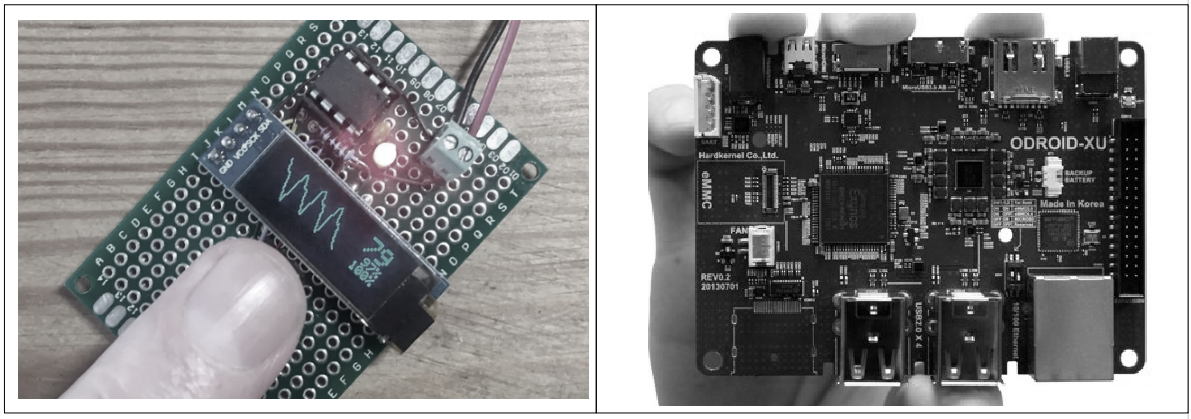
\includegraphics[scale=0.25]{images/microvssoc.png}
\caption{Dos sistemas embebidos. A la izquierda sencillo con MCU (microcontrolador). A la derecha otro mas complejo con un SoC (System-On-Chip)}
\label{fig:microvssoc}
\end{figure}



Los microcontroladores suelen tener un software que fue 
desarrollado con los drivers mínimos necesarios. Esto los hace
muy eficiente al momento de controlar Entradas y Salidas
en momentos exactos. 

\subsubsection{Microcontrolador AVR de 8 bits}

Las arquitecturas de CPU mas comunmente usadas en microcontroladores
son PIC, AVR, 8051 y 68000; siendo las primeras 3 ampliamante usadas
en toda clase de dispositivos.

Para nuestros laboratorios utilizaremos microcontroladores AVR de 8 bits,
por un buen número de razones. Una vez avanzados en la práctica
estas razones serán obvias. Los AVR son una familia de microcontroladores de 8 bits, con arquitectura
RISC, que fue diseñada desde un comienzo 
para la ejecución eficiente de código C compilado\footnote{https://www.microchip.com/design-centers/8-bit/avr-mcus}. Debido a que
la ejecución de las instrucciones más comunes se dan en un sólo
ciclo de reloj, los microcontroladores AVR alcanzan un rendimiento
de 1 MIPS por Mhz de reloj, permitiendo a los diseñadores de
sistemas optimizar el consumo de energía versus la velocidad
de procesamiento requerida.

Como ejemplo describiremos el microcontrolador AVR atmega328, 
el cual es muy utilizado en las placas
Arduino. Este microcontrolador trae tres tipos de memoria on chip: 2KB de memoria \textbf{RAM},
32KB de memoria \textbf{FLASH} y 1KB de memoria \textbf{EEPROM}.

En cuantos a los periféricos de E/S se puede mencionar:
varias líneas de E/S de propósito general (\textbf{GPIO}), un conversor
analógico a digital (\textbf{ADC}), interfaces seriales para comunicación 
\textbf{UART}, interfaces seriales \textbf{I2C} y \textbf{SPI} para conectar 
dispositivos externos, interrupciones, \textbf{timers}, y 
salidas \textbf{PWM} conectadas a estos relojes.

Para su programación exiten diferentes compiladores de C
y otros lengujaes. En particular el compilador de C
del proyecto \textbf{GNU GCC} es el más ampliamante usado,
y es el estándar en la industria. Está conformado
por el compilador de C, la biblioteca de C estándar,
un ensamblador, un vinculador, un debugger, y herramientas de 
manejos de archivos binarios y de objetos (por ejemplo,
un desemsamblador)\footnote{https://gcc.gnu.org/wiki/avr-gcc}\footnote{https://www.nongnu.org/avr-libc/}. Para transferir los programas al 
chip se utiliza general la herramienta avrdude\footnote{https://www.nongnu.org/avrdude/}.
Todo este software se encuentra disponible para los sistemas
operativos Windows, Mac y Linux.

Los microcontroladores AVR ya traen incorporado una interfaz
de programación serial que requiere de un hardware mínimo
de interconexión.





\pagebreak

\section{Referencias}

Michael Barr. Programming Embedded Systems in C and C++ 1st Edition. ISBN-13: 978-1565923546
ISBN-10: 1565923545. O'Reilly Media; 1 edition (February 9, 1999)


\section*{Licencia y notas de la traducción}

Rafael Ignacio Zurita ({\texttt{rafa@fi.uncoma.edu.ar}) 2016-2020

Este apunte es una traducción del libro de referencia, para
ser utilizado como apunte en la materia de grado
'Programación de Sistemas Embebidos' de la Facultad de Informática,
Universidad Nacional del Comahue.
Se han realizado modificaciones
al contenido para aclarar ciertos detalles o agregar secciones nuevas.
 Tambien se han
modificado todos los archivos fuentes de código, ya que fueron
portados a la plataforma Atmel AVR atmega328.


\fcolorbox{black}{cyan}{
\parbox[t]{1.0\linewidth}{ \vspace*{0.4cm}
Esta es una obra derivada del libro de referencia que ha obtenido permiso de O'Reilly para su publicación en PEDCO.
\vspace*{0.4cm} } }

\subsubsection{Permiso de publicación}

\begin{small}
\begin{verbatim}
From: Teri Finn <teri@oreilly.com>
Date: Mon, 11 Apr 2016 15:48:58 -0700
Message-ID: <CAOgscZ92-G9iT+=+nnuft4LCoHoe5o8SYPfVEKnS6AKXh8TLyQ@mail.gmail.com>
Subject: Re: Question about permission to translate some parts
To: Rafael Ignacio Zurita <rafa@fi.uncoma.edu.ar>
Content-Type: multipart/alternative; boundary=94eb2c094eeedeba0005303d5a31

--94eb2c094eeedeba0005303d5a31
Content-Type: text/plain; charset=UTF-8

Hi Rafael,

Thank you for providing this further information.  O'Reilly Media is happy
to grant you permission to translation the content you have proposed for
posting to the Moddle site. We're happy you find this information helpful
to the students.

Best regards,

Teri Finn
O'Reilly Media, Inc.

On Thu, Apr 7, 2016 at 10:56 AM, Rafael Ignacio Zurita <
rafa@fi.uncoma.edu.ar> wrote:

[snip]
\end{verbatim}
\end{small}



%\end{otherlanguage}
% } % foreign language


\end{document}


